\chapter{Technologies}
\thispagestyle{pagestyle}

Pie's technologies were chosen with maintainability in mind. I have integrated various technologies and third-party libraries already used in popular mature open-source projects. Such technologies are backed up by large communities and frequent updates, confirming that they will not become obsolete in the near future.

\section{Microsoft's Windows Forms and the .NET Framework}

THE .NET Framework was introduced in 2001 by Microsoft, together with the Visual Studio tool. It was built for the purpose to simplify Windows application development \cite{net-framework}, currently supporting three languages, also developed by Microsoft: Visual Basic, a user interface adaptation of the BASIC language, C\#, and F\#.

Pie uses Windows Forms (commonly referred to as "WinForms"), as the primary technology for its graphical user interface and business logic. WinForms is a technology that was introduced with the first version of .NET. It "can be thought of as a wrapper around the complex Win32 API" \cite{winforms-history}. The solution 
simplified desktop development by allowing programmers to focus on the business logic, instead of coding user interface components. Components, officially known as "Controls", could be added to application windows (or "Forms") simply by dragging and dropping them on the workbench.

Although not the first WYSIWYG ("What You See Is What You Get") designer, Windows Forms is certainly one of the most popular ones, as it came directly from Microsoft, the developer of Windows, receiving frequent updates and support even to this day. It is also available for all of the three .NET languages. I have chosen C\#, as it is the most commonly used among them.

WinForms is not the only user interface technology developed by Microsoft. Several years later, in 2006, Windows Presentation Foundations ("WPF") has been introduced, followed by the Universal Windows Platform ("UWP") technology in 2015. Although the latter provide a more actual way of splitting user interface logic and business logic, Windows Forms received more support during the years, is simpler to use, and has more compatible extensions ready to be integrated. Windows Forms is also considered to be a better option, from a memory management point of view. Performance is also a key to be taken into consideration, and in this manner, it seems that there is no significant difference between newer technologies such as WPF and WinForms \cite{han2023optimization}. Even so, the Form components inside Pie do not incorporate a large number of controls (e.g. buttons, textboxes, labels, panels) and the file handling logic is as simple and possible, using actual C\# integrated methods. Thus, the application is not expected to cause any slow-downs during the start-up or the usage of it.

The "Form" control is a representation of any window displayed in an application. The Form class can be used to create standard, floating and borderless windows. The "Properties" panel (present in any type of Control object), can be used to determine the appearance, size, color and window management features of the windows or dialog boxes that are created. \cite{form-class}

\begin{figure}[H]
\centering
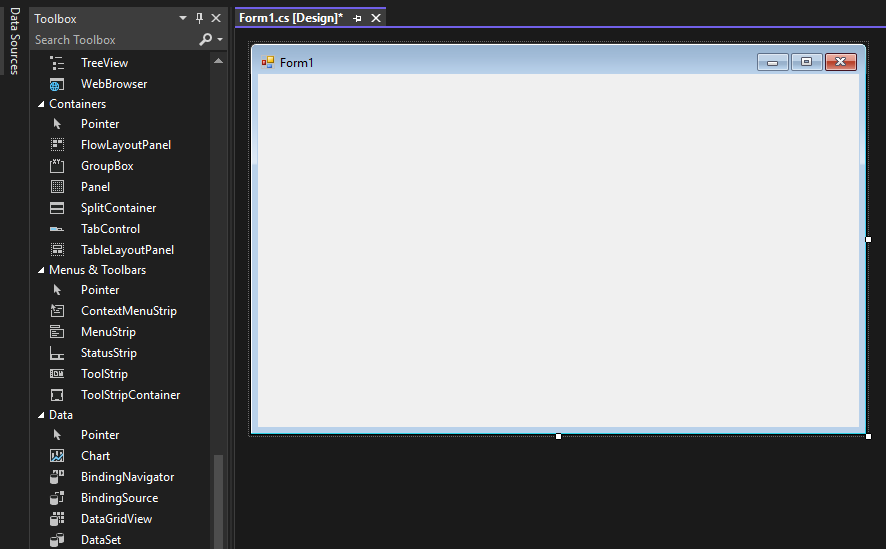
\includegraphics[width=0.8\textwidth]{images/winforms-designer.png}
\caption{Designing a Form using the WinForms technology in Visual Studio}
\label{fig:fig2,1.}
\end{figure}

Controls (available in the "Toolbox" sidebar of the designer) can have certain "Events" attached to them. Events can be triggered on several occasions:

\begin{enumerate}
  \item a mouse is hovered over the control;
  \item the control is clicked;
  \item someone presses a key, while holding focus on the control. 
\end{enumerate}

Pie uses a large number of event handlers, being able to respond to certain key bindings accordingly. Thus, users can toggle different user interface components such as the Find\&Replace dialog or the integrated terminal system simply by pressing a predefined key combination. 

The NuGet pacakge manager, integrated into Visual Studio, is the most effective and secure way to add external libraries to a .NET project. It provides a large collection of packages built by developers, including file parsers, user interface components, or database drivers, ready to be bundled into the application.

\begin{figure}[H]
\centering
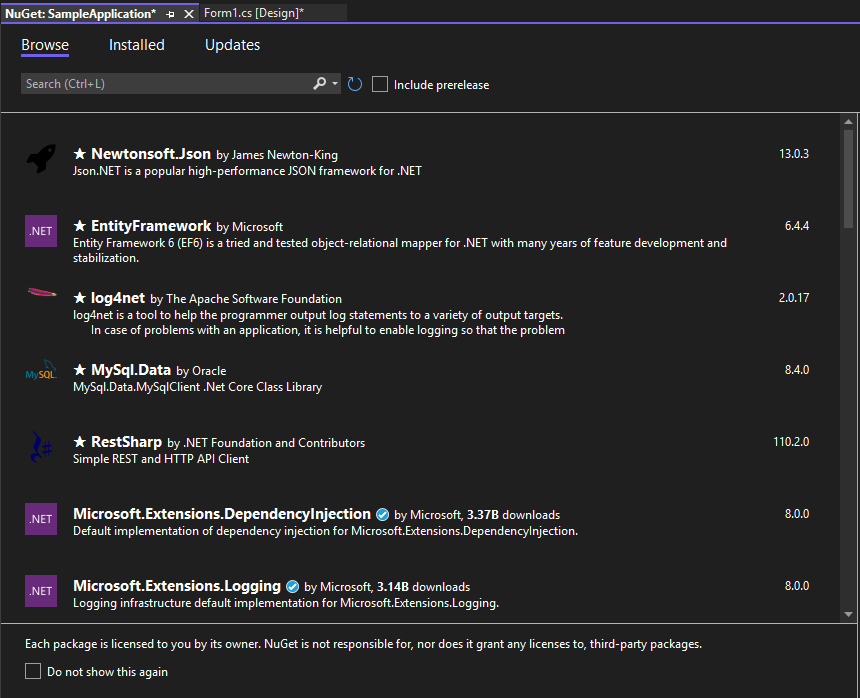
\includegraphics[width=0.8\textwidth]{images/nuget.png}
\caption{Using NuGet to discover packages available to install in a Windows Forms application}
\label{fig:fig2,1.}
\end{figure}

\section{Third-party libraries included with Pie}
\subsection{Redesigning .NET components with Krypton and ObjectListView}

Even though WinForms offers a vast toolbox of controls and customization options, it still has its limitations when it comes to design of native Windows elements. While most of the components can be customized, this typically requires writing complex event handling logic and overriding methods from the framework's base classes. In order to minimize the default Windows look in my application, I have integrated a third-party library called Krypton \cite{krypton}.

Krypton provides a better way to personalize the overall design of WinForms controls through the integration of the "KryptonPalette" class. A singleton instance of this class is accessible from all components in the application, including forms, panels, buttons, and labels. I have defined a general color scheme and other design aspects, such as border rounding and label font size, and have configured all project components to inherit their properties from this singleton.

Another limitation of Windows Forms is the ListView control. A ListView is used to display multiple elements in a list \cite{listview}, being able to handle events such as mouse clicks, mouse hovers, and key presses. However, neither the native ListBox integrated into Visual Studio nor Krypton's implementation of the ListView offers the level of customization needed for my application. To address this, I have integrated the ObjectListView \cite{objectlistview} library into the project.

ObjectListView allows for the mapping of actual objects (not just strings) to ListView controls, and offers a way to assign icons or specific colors to each element based on specific fields. This "Object-to-ListView" mapping was a requirement for Pie, as the control is used to display the status of the files in Git repositories, the list of custom build commands, and the database connections added to the application.

\subsection{Relying on Newtonsoft.Json to parse configuration files}

Pie stores configuration files such as color scheme definitions and Git credentials in JSON-formatted files. JSON is preferred over popular formats like XML, when simple data is transmitted, and the focus is on the data handling performance \cite{json-vs-xml}.

Whenever the user does a change in the configuration of the application, a JSON file needs to be rewritten. In the same manner, whenever Pie is started, the entire configuration specified in the JSON files needs to be loaded internally. A proper way of handling these files is through the Newtonsoft.Json \cite{newtonsoft-json} parsing library.

Newtonsoft.Json is used to deserialize (read) JSON files into internal configuration objects and to serialize (write) these objects back into JSON files in an efficient manner, without introducing any noticeable temporal overhead.

\subsection{Integrating the code editing functionality with Scintilla}
\subsection{Terminal instance management using ConEmu}
\subsection{Using CefSharp and Markdig for rendering code inside web browsers}
\subsection{Managing Git repositories with LibGit2}
\subsection{Querying databases with various SQL drivers}